\documentclass[a4paper]{article}
\usepackage[top=2cm, bottom=2cm, left=2cm, right=2cm]{geometry}

\usepackage[T1]{fontenc}
\usepackage[utf8]{inputenc}
\usepackage{amsthm}
\usepackage{graphicx}          % To handle figures
\usepackage{amsmath}           % Defines certain mathematical symbols
\usepackage{amsfonts}


\renewcommand{\thesubsection}{\arabic{section}.\alph{subsection}}

\begin{document}


%---------------------------------------------------------------------------------------------------------
%Title
\newcommand{\HRule}{\rule{\linewidth}{0.5mm}} 
\title{{\LARGE EQ2410 - Advanced Digital Communications} \\[0.5cm] \HRule \\[0.4cm]{Project 2 : LDPC Decoding}\\[0.2cm] \HRule \\[0.5cm] }
\author{Baptiste Cavarec \\ 940321-T197 \and Hugo Lime\\  920707-4635 \and Adrien Anxionnat\\ 921128-T218}
%\date{2000-10-10}

\maketitle
\abstract
In short introduction, we all gathered together to work on this project, so that every personal knowledge is shared and transformed into a group work. In this report you can find our results on the exercises 1 and 2.
%---------------------------------------------------------------------------------------------------------
%Problem 1
\section{Problem 1}
\subsection{Presentation of the problem}
We were given a program simulating a transmission system using LDPC coding mapped to BPSK. Our main task was first to identify the channel, the system components and do simulations to estimate the bit-error rate of this given channel.
\subsection{Identification of transmission system}

By reading the matlab code main.m one can see that the channel is represented as: $e(i)= 1-2*(rand<\epsilon);$ where $rand<\epsilon$ is a boolean hence it tranforms b in -b with the probability $\epsilon$ so the channel represented by the equation is a Binary Symmetric Channel (BSC).
As it is a BSC channel it is sufficient to consider the all zero codeword as the swap is independent of the bit value (0 or 1) so only considering this word is sufficient to quantize the performance of our decoder.\\

The Algorithm used here in order to decode the LDPC is Gallager's Algorithm A, one can recognize the variable node implemented in decoder\_1 (if all the other nodes point to -y then its -y else we keep y) and the check node implemented in decoder\_2 (the sum is mapped to a product in BPSK and then vi is the product of all the other elements)
By looking in the matlab code and workspace it is easy to find out that Distr1a is of degree 3 then Distr2a is of degree 6 and Distr1b is of degree 3 and lastly Distr2b is of degree 6.\\

When generating the check matrix for a fixed length of codeword, it may not be possible to get the exact edges distribution we want because we need an integer number of nodes. This problem is solved in \verb|main.m| by adjusting the number of nodes for each degree to get as close as possible to the desired distribution (see added comments in the program).

\section{Problem 2}
\subsection{Presentation of the problem}
The idea is now to change the transmission system in order to make it fit onto a Binary Erasure Channel (BEC). Our first task is to transform the equations of the channel (that was previously a BSC). In order to map or channel to a BEC we simply encode the erasure channel as:  $e(i)= 1-(rand<\epsilon);$ then it maps the bit b $\in \{-1,+1\}$ into either b or 0 with the probability $\epsilon$.

\subsection{The belief-propagation decoder }

The next step in order to implement a channel decoder is to implement the belief propagation decoder. Instead of transmitting the bits we transmit the log likelihood ration (LLR).
An usual measurement is to take $u_0= log( \frac{Pr(x=1|y)}{Pr(x=-1|y)})$ the issue with the following measure is that in the case of the BEC if the channel sends $y=-1 $ or $y=1$ the probability are 0 or 1 hence the logarithm is not defined. A more appropriate measure in our case  is to consider $u_0= Pr(x=1|y)-Pr(x=1|y)$ since $Pr(x=-1|y)=1-Pr(x=1|y)$. Then $u_0=2*Pr(x=1|y)-1$
This leads to the following possibilities : $u_0=1$ when $y=1$, $u_0=0$ when $y=0$ and $u_0=-1$ if $y=-1$.

Then the check nodes calculate their response $u_{ij}=\prod_{k \neq i}{v_{kj}}$. One may notice that $u_{ij}=0$ if there is any erased bit.
Then the variable node always sends $u_0$ if $y \in \left\{-1,1\right\}$ (there is no swap) else if there is $j$ so that $u_{ij} \neq 0$ then $u$ is set to $u_{ij}$.

\subsection{Density evolution}

Since a correct node won't be changed by the decoder, the only nodes that will evolve through time are the erasure nodes that have note been decoded. Hence, to perform density evolution it is necessary and sufficient to follow the erasure probability exchanged by the nodes.

Let's consider a degree $d_v$ variable node, for it to send an erasure message at state $n$ it must be that it was initially an erasure (probability $\epsilon$) and that it received erasure messages from all the $d_v-1$ check nodes (probability $q(n-1)^{d_v-1}$) then we easily find : 
\begin{equation}
p(n)=\epsilon q(n-1)^{d_v-1}
\label{eq1}
\end{equation}
Let's consider a degree $d_c$ check node, for it to send an erasure message at state $n$ it must be that one of the other variable node sent an erasure message. Hence it is correct only if all the $d_c-1$ nodes send no erasure message ( that happens for one node with probability $1-p(n-1)$) then the overall probability of having everything right is $(1-p(n))^{d_c-1}$ then the overall probability of sending an erasure is:

\begin{equation}
q(n)= 1-(1-p(n))^{d_c-1}
\label{eq2}
\end{equation}
%Combining Eq.~\ref{eq1} and Eq.~\ref{eq2} gives us the probability that a node remains erased at time $n$ is given by :
%\begin{equation}
%p(n)= \epsilon (1-(1-p(n-1))^{d_c-1})^{d_v-1}
%\label{eq3}
%\end{equation}

Let's note Eq.~\ref{eq1} $p(n)=f(q(n-1))$ and Eq.~\ref{eq2} $q(n)=g(p(n))$ %then Eq.~\ref{eq3} can be written $p(n)=f \circ g(p(n-1))=h(p(n-1))$.
%Then as $h\in C^2$ the recurrence sequence $\{p\}_{n\in\mathbb{N}}$ converges if and only if there exist $l$ so that $h'(x)\leq l <1$ and then the sequence converges to the unique fixed point of h (in our case 0). %Je crois que c'est pas le bon th�or�me, son crit�re est pas n�c�ssaire je crois
In order for our sequence $\{p\}_{n\in\mathbb{N}}$ to converge to 0 it must be strictly decreasing  then $p(n+1)<p(n)$ then $ f(q(n))<g^{-1}(q(n))$ as $q(n) =g(p(n))$.

Then $ \epsilon q^{d_v-1}<1-(1-q)^{\frac{1}{d_c-1}}$. 

We then can write $ \epsilon<\frac{1-(1-q)^{\frac{1}{d_c-1}}}{q^{d_v-1}}$, then for the (3,6) LDPC  $ \epsilon<\frac{1-(1-q)^{\frac{1}{5}}}{q^{2}}$

%We can derive in order to find the minimum of the function: $\frac{d}{dq} \frac{(1-(1-q)^{1/5})}{q^2} = \frac{-9 q-10 (1-q)^{4/5}+10}{5 (1-q)^{4/5} q^3}$
%It is equal to 0 when $q\approx 0.77895$ which gives $ \epsilon_T \approx 0.42944 $.
We need this condition to be valid for $q \in [0,\frac{1}{2}]$ which gives $ \epsilon_T \approx 0.5178 $. It is confirmed by Figure \ref{bec} and Figure \ref{fandg}.

\begin{figure}[ht!]
\centering
\begin{center}
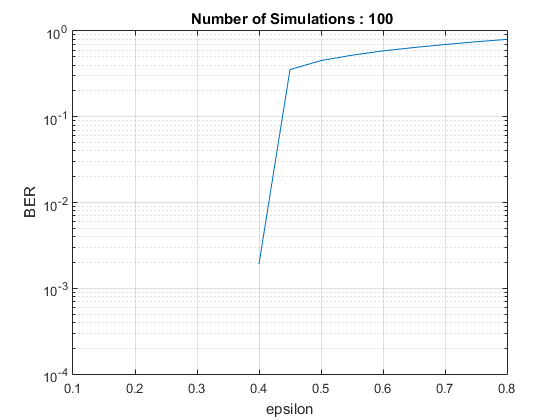
\includegraphics[scale=0.70]{bec.png}
\caption{Erasure probability, it shows that the decoder converge for $\epsilon < 0.5$}
\label{bec}
\end{center}
\end{figure}

\begin{figure}[ht!]
\centering
\begin{center}
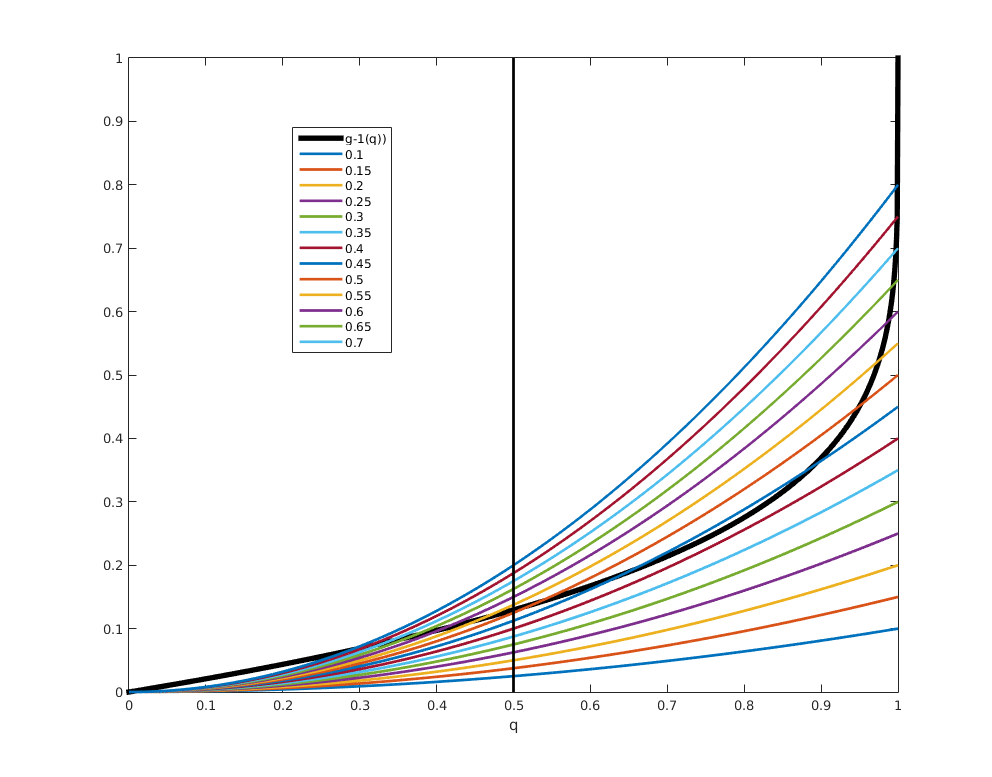
\includegraphics[scale=0.60]{fandg2.png}
\caption{functions $f$ for different values of $\epsilon$ compared to $g^{-1}$}
\label{fandg}
\end{center}
\end{figure}

\end{document}